\section{Software} \label{sec:software}

\subsection{Klassendiagramm} \label{subsec:klassendiagramm}

\begin{figure}[H]
	\begin{minipage}[h]{0.45\linewidth}
		\centering
		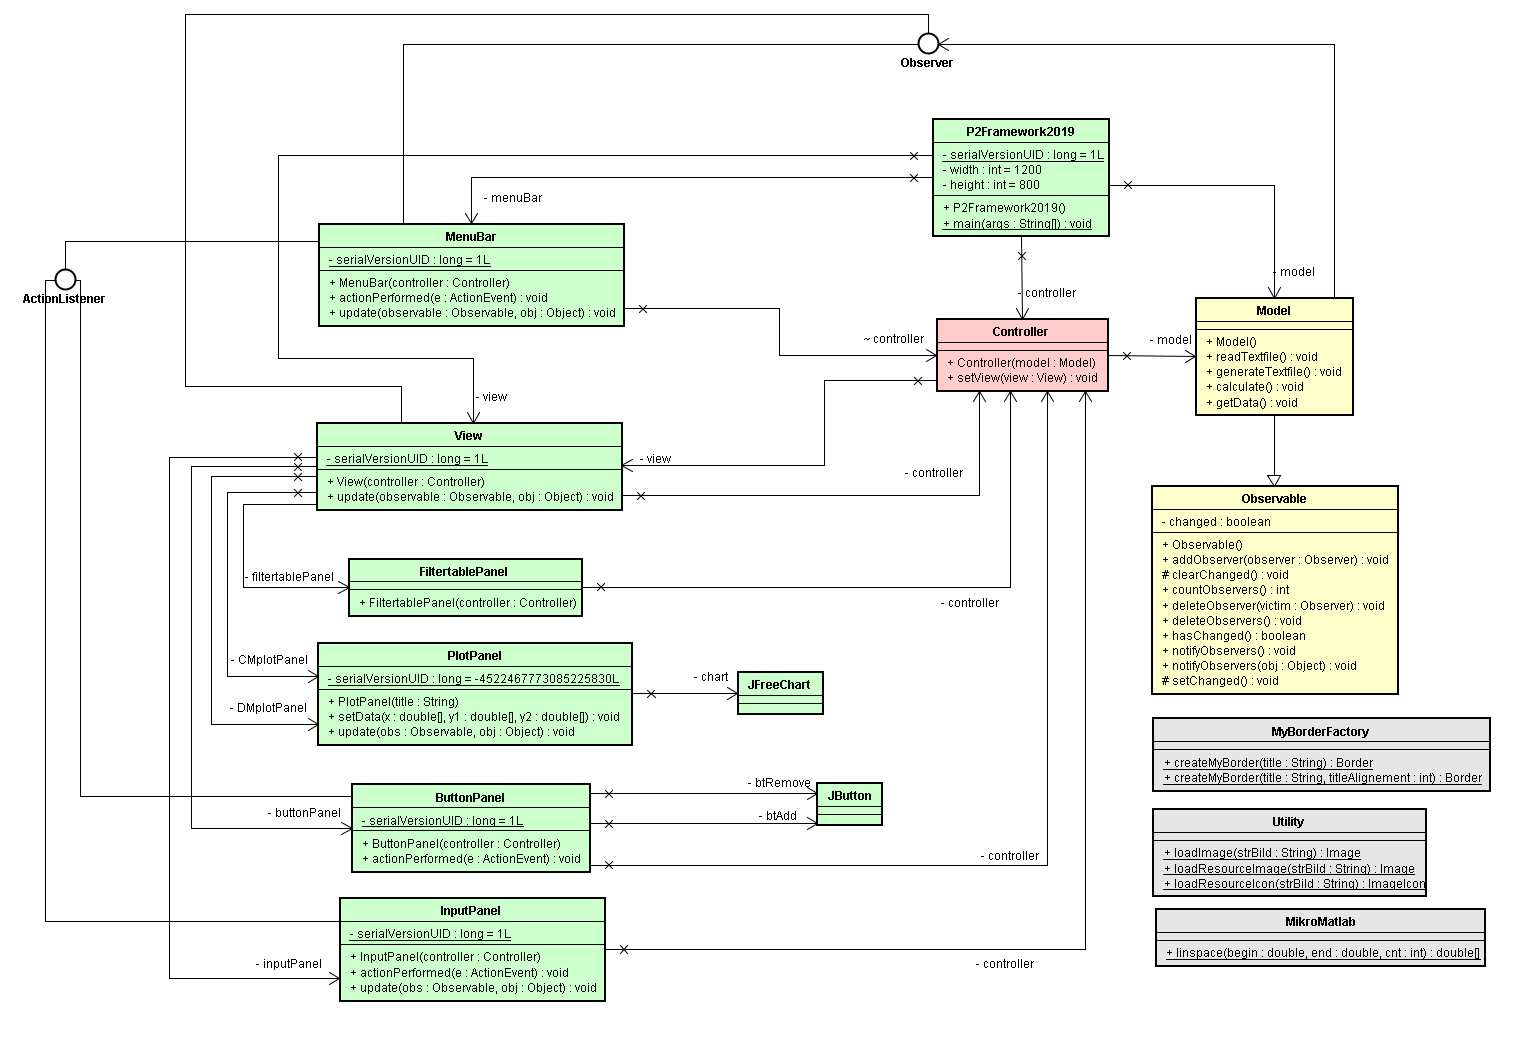
\includegraphics[width = 18cm]{Klassendiagramm.png}
		\label{fig:piImpedance}
		\caption{Klassendiagramm \cite{wtf}}
	\end{minipage}
\end{figure}

\subsection{Ersatzschaltbilder} \label{subsec:ersatzschaltbilder}

\begin{figure}[H]
	\begin{minipage}[h]{0.45\linewidth}
		\centering
		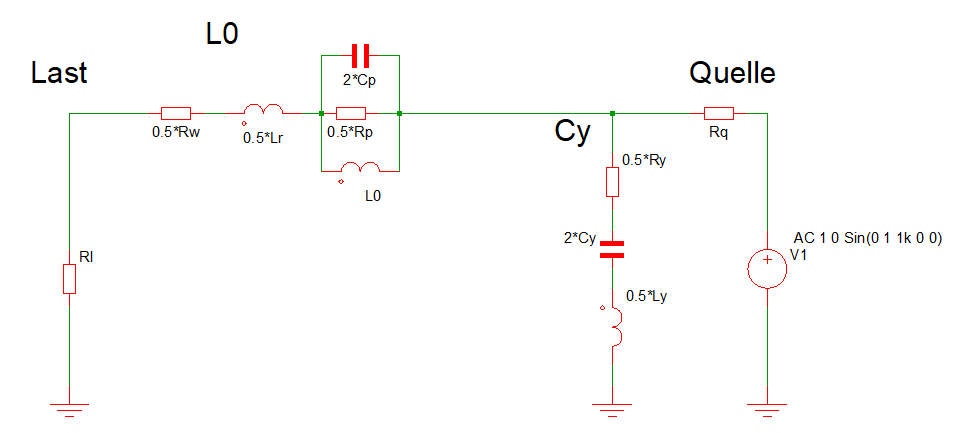
\includegraphics[width = 6cm]{EMI_CM.png}
		\label{fig:piImpedance}
		\caption{Vereinfachte \cite{CM_Schaltung}}
	\end{minipage}
\end{figure}


\begin{figure}[H]
	\begin{minipage}[h]{0.45\linewidth}
		\centering
		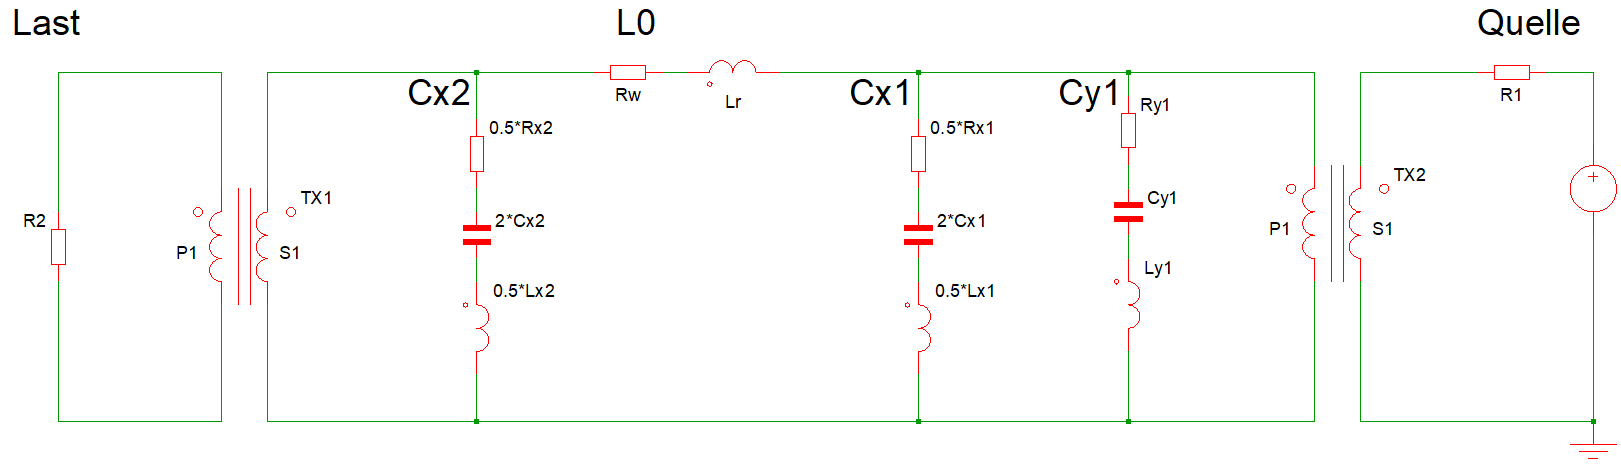
\includegraphics[width = 6cm]{EMI_DM.png}
		\label{fig:piImpedance}
		\caption{Vereinfachte \cite{DM-Schaltung}}
	\end{minipage}
\end{figure}

\subsection{GUI} \label{subsec:gui}



\subsubsection{Menu}\label{menu}


\subsection{Datenverarbeitung} \label{subsec:datenverarbeitung}



\subsection{Datenpräsentation} \label{subsec:datenpräsentation}



\subsection{Speicherverwaltung} \label{subsec:speicherverwaltung}

Programmablauf beschreiben?



